%%%%%%%%%%%%%%%%%%%%%%%%%%%%%%%%%%%%%%
% P R O F I L E
%%%%%%%%%%%%%%%%%%%%%%%%%%%%%%%%%%%%%%
\begin{facts}
    % \adjustbox{valign=t}{
    % \begin{tikzpicture}[scale=0.85]
    %     \filldraw[fill=imageborder] (0,0) circle (2.7cm);
    %     \clip (0,0) circle (2.5cm);
    %     % \node[anchor=center] at (0, 0.25) {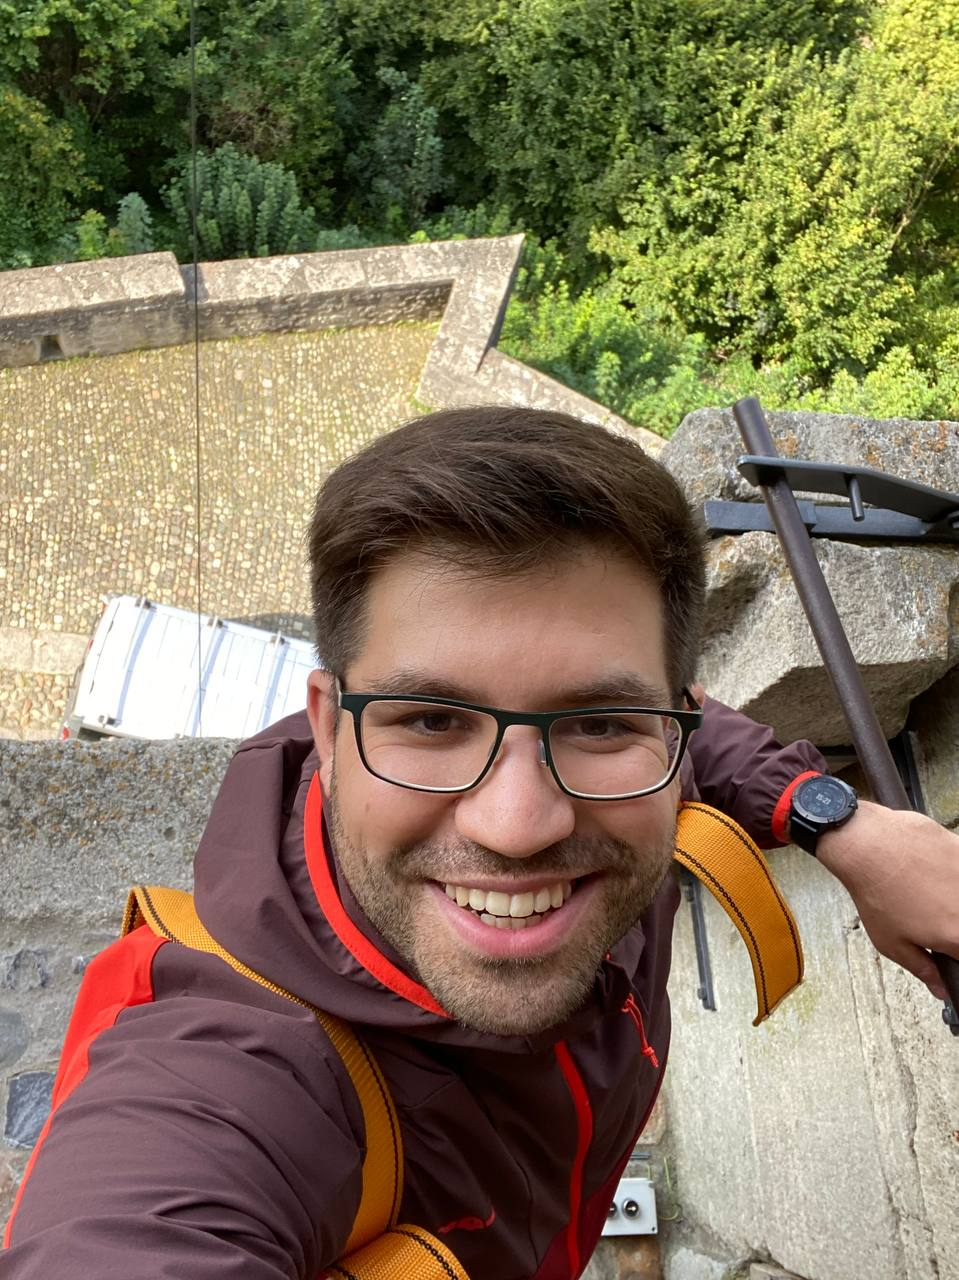
\includegraphics[width=4.5cm]{images/me}}; 
    %     %adjust this coordinate to move image
    % \end{tikzpicture}
    % }
    % \adjustbox{valign=t}{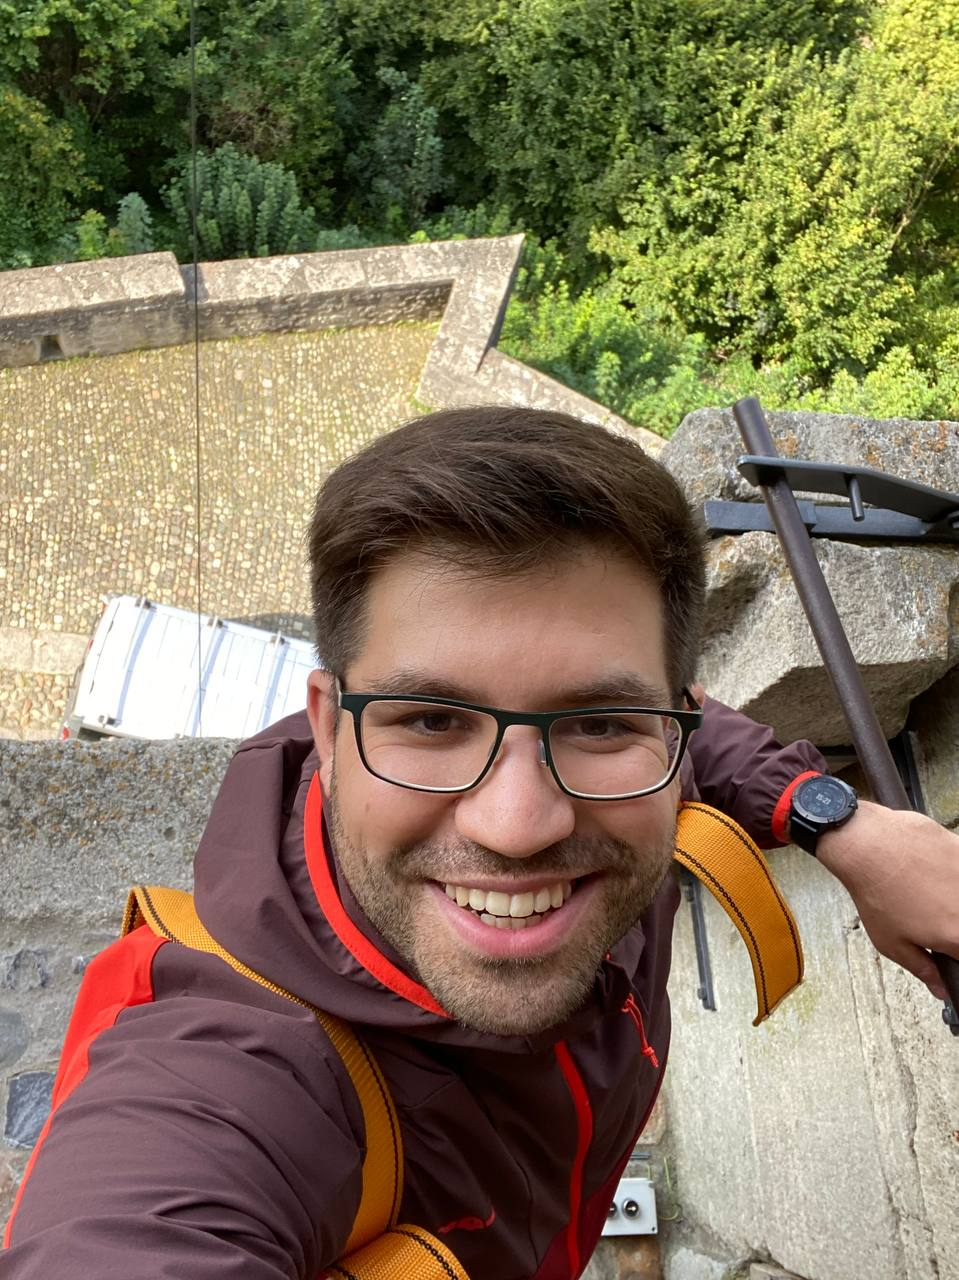
\includegraphics[width=0.85\textwidth,clip,cfbox=heading 0pt 0pt]{images/me}} % trim={1.4cm 5.4cm 1.95cm 0.8cm}
    % \sectionsep
    \section{Noah Hüsser}
    Nationality: Swiss\\
    % Date of Birth: 12th January 1991
    \sectionsep
    
    \subsubsection{Contact}
    noah@huesser.dev\\
    +41 79 960 7130\\
    \href{https://github.com/Yatekii}{https://github.com/Yatekii}\par
    \vspace{\baselineskip}
    Ammerswilerstrasse 31F\\
    5600 Lenzburg\\
    Switzerland
    \sectionsep
    
    \subsubsection{Activities}
    Programming, Electronics,\\
    Server Admin, Ju Jitsu, \\
    Running
    \sectionsep
    
    %%%%%%%%%%%%%%%%%%%%%%%%%%%%%%%%%%%%%%
    % S K I L L S
    %%%%%%%%%%%%%%%%%%%%%%%%%%%%%%%%%%%%%%
    \subsubsection{Professional Skills}
    Software Development\\
    SRE\\
    Project Management\\
    Embedded Systems
    \sectionsep
    
    \subsubsection{Languages}
    German \describe{mother tongue}\\
    English \describe{fluent}\\
    French \describe{experienced}
    \sectionsep
    
    \subsubsection{Engineering Tools}
    Linux/Unix Administration\\
    Docker, K8S\\
    GL CI, GH Actions\\
    Jupyter, Scipy, Numpy, Pandas
    \sectionsep
    
    \subsubsection{Programming}
    \describe{frequently used}\\
    Rust, Dart, Python, C, C\#,\\
    JavaScript, SQL
    \sectionsep
    
    \describe{used in the past}\\
    VHDL, Tcl, Java, PHP, C++,\\
    Bash, VB.NET, LaTeX
    \sectionsep
    
    \subsubsection{Miscellaneous}
    Git
    \sectionsep
    
    \subsubsection{References}
    on request
    
    \sectionsep
    Last updated \today.
    
    \end{facts}%
    \begin{timeline}
    
    %%%%%%%%%%%%%%%%%%%%%%%%%%%%%%%%%%%%%%
    %     EXPERIENCE
    %%%%%%%%%%%%%%%%%%%%%%%%%%%%%%%%%%%%%%
    
    \subsection{Practical Experience}

    \subsubsection{Cryptocurrency Exchange}
    \meta{Contractor, Rust Backend Engineer}{December 2021}{Present}{Zürich}
    Maintainer of the biggest internal microservice.
    Focus on stability, developer experience and fast \& easy integration testing as well as CI performance.
    \sectionsep
    
    \subsubsection{Technokrat}
    \meta{Co-Founder, Software Engineer}{May 2017}{October 2021}{Zürich}
    Co-founded a consulting company for electrical engineering. Realizing software from embedded devices to cloud services and webapplications.
    \sectionsep

    \subsubsection{Siglis}
    \meta{Co-Founder, Software Engineer}{August 2020}{August 2021}{Zürich}
    Founded a smart home company which develops a smart switch (\href{https://zigfred.ch}{zigfred.ch}).
    Developing and manufacturing a product from start to finish. Responsibilities included mechanical design, mobile app and automated factory testing and provisioning.
    \sectionsep

    \subsubsection{ABB Micafil}
    \meta{Part Time Software Engineer}{Jul 2016}{March 2018}{Zürich}
    Development of a CAD tool to dimension bushings in VB.NET.
    Development of a system to monitor, analyze and control the production line of a bushing.
    \sectionsep
    
    \subsubsection{Nexus Telecom}
    \meta{Low Level C Programmer}{Mai 2014}{Mai 2015}{Zürich}
    Porting the core C library from 32 to 64 bit.
    \sectionsep

    %%%%%%%%%%%%%%%%%%%%%%%%%%%%%%%%%%%%%%
    %     VOLUNTEER EXPERIENCE
    %%%%%%%%%%%%%%%%%%%%%%%%%%%%%%%%%%%%%%
    
    \subsection{Volunteer Experience}
    
    \subsubsection{Ju Jitsu Club Aarau}
    \meta{Treasurer}{Apr 2019}{present}{Aarau}
    \sectionsep

    \subsubsection{Bastli, Students Lab, ETH Zurich}
    \meta{President}{Feb 2016}{Oct 2016}{Zürich}
    \meta{Treasurer}{Feb 2015}{Feb 2016}{Zürich}
    \sectionsep

    %%%%%%%%%%%%%%%%%%%%%%%%%%%%%%%%%%%%%%
    %     EDUCATION
    %%%%%%%%%%%%%%%%%%%%%%%%%%%%%%%%%%%%%%
    
    \subsection{Education}
    
    \subsubsection{FHNW Brugg-Windisch}
    \meta{BsC in EE and IT}{Feb 2016}{Jan 2017}{Windisch}
    \sectionsep
    
    \subsubsection{ETH Zürich}
    \meta{BsC in EE and IT}{Sep 2013}{Feb 2016}{Zürich}
    \sectionsep
    
    %%%%%%%%%%%%%%%%%%%%%%%%%%%%%%%%%%%%%%
    %     PUBLICATIONS
    %%%%%%%%%%%%%%%%%%%%%%%%%%%%%%%%%%%%%%
    
    \subsection{Publications and Open Source}

    \subsubsection{probe-rs embedded toolchain}
    \meta{Project Lead}{Mar 2019}{present}{\href{https://probe.rs}{probe.rs}}
    The toolkit allows to control embedded ARM and RISC-V MCUs to be controlled from a host.
    The project offers:\\
    \begin{tightemize}
    \item a libray to control targets from code
    \item CLI tools to flash and log data from targets
    \item A VSCode debugger plugin
    \end{tightemize}
    \sectionsep
    
    \subsubsection{FPGA Based Spectrum Analyzer}
    \meta{Bachelor Thesis at FHNW}{Mar 2017}{Aug 2017}{Windisch}
    The tasks included, but were not limited to, the implementation of:
    \begin{tightemize}
    \item CIC/FIR-filter-chains for data decimation
    \item A server to transmit data via WebSockets on an embedded Linux
    \item A GUI to retrieve data over WebSockets, transform and display it (JavaScript)
    \end{tightemize}
    \sectionsep
    
    % \subsubsection{FPGA Based Oscilloscope}
    % \meta{Group Thesis at ETH Zürich}{Sep 2015}{Dec 2015}{Zürich}
    % The tasks included, but were not limited to, the implementation of:
    % \begin{tightemize}
    % \item Recursive trigger logic to detect special signal patterns (VHDL)
    % \item Kernel module for data reading and processing on an ARM Core A9 (C)
    % \item GUI to retrieve data over TCP/IP, filter and display it (C++, Python, Qt5)
    % \end{tightemize}
    % \sectionsep

    \end{timeline}%